\documentclass[letter]{article}

\usepackage[english]{babel}
\usepackage[utf8]{inputenc}
\usepackage{amsmath}
\usepackage{graphicx}
\usepackage[colorinlistoftodos]{todonotes}
\usepackage{makecell}
\usepackage{multirow}
\usepackage{caption}
\usepackage{hyperref}
\usepackage[all]{hypcap}
\usepackage{enumitem}

\newlist{questions}{enumerate}{1}
\setlist[questions, 1]{label = \arabic*}
\newlist{bonus}{enumerate}{1}
\setlist[bonus, 1]{label = Bonus \arabic*}


% Adjust margins
\addtolength{\oddsidemargin}{-0.375in}
\addtolength{\evensidemargin}{-0.375in}
\addtolength{\textwidth}{1in}
\addtolength{\topmargin}{-.5in}
\addtolength{\textheight}{1.0in}

\title{CS 520: Assignment 1 - Path Planning and Search Algorithms}

\author{Shengjie Li}

\date{\today}

\begin{document}
\maketitle

\section{Introduction, group members and division of workload}
\label{sec:Introduction}

In this group project, apart from implementing DFS, BFS, $ A^* $ with Euclidean Distance and $ A^* $ with Manhattan Distance, we also did some modification to these algorithms for different performance out of our personal interests.  \\
\begin{tabular}{| p{2.5cm} | p{11.5cm} |}
	\hline
	\makecell[c]{Name \\ RUID} & Workload \\
	\hline
	\makecell[c]{Haoyang Zhang \\ 188008687} & {Implemented DFS, Iterative Deepening DFS, BFS, Bidirectional BFS, Beam Search, Simulated Annealing and the visualization of maze. Modified DFS to make it able to return optimal path. Added Last-in First-out feature to $ A^* $. Managed to combine Beam Search, Simulated Annealing and Genetic Algorithm. Ran tests for DFS and BFS in question 10. Finished half of the writing of report for part 2.} \\
	\hline
	\makecell[c]{Han Wu \\ 189008460} & {Wrote python scripts for testing the performance of algorithms. Got and Combine the data for question 1, 2, 4 and 5. Finished the writing of report for question 1, 2, 4 and 5.} \\
	\hline
	\makecell[c]{Shengjie Li \\ 188008047} & {Implemented $ A^* $ with Euclidean Distance, $ A^* $ with Manhattan Distance and Genetic Algorithm. Ran tests for $ A^* $ with Euclidean Distance and Manhattan Distance inquestion 10. Finished the writing of whole report. } \\
	\hline
	\makecell[c]{Zhichao Xu \\ 188008912} & {Wrote python scripts for testing the performance of algorithms. Got and Combine the data for question 3, 6 and 7. Generated figures for questions in part 1. Finished the writing of report for question 3, 6 and 7. Suggested an improvement of $ A^* $ using Chebyshev Distance.} \\
	\hline
\end{tabular}


\section{Part 1: Path Planning}
\label{sec:Part 1: Path Planning}

\begin{questions}
	\item {For each of the implemented algorithms, how large the maps can be ( in terms of dim ) for the algorithm to return an answer in a reasonable amount of time (less than a minute) for a range of possible p values? Select a size so that running the algorithms multiple times will not be a huge time commitment, but that the maps are large enough to be interesting.} \\
	The results are shown below as Table \ref{Table 1}: \\
	\begin{center}
		\label{Table 1}
		\begin{tabular}[h]{| c | c | c | c | c | c | c | c |}
			\hline
			\multicolumn{2}{|c|}{} & \multicolumn{6}{c|}{Size} \\
			\cline{3-8}
			\multicolumn{2}{|c|}{} & 100 & 200 & 400 & 800 & 1600 & 3200 \\
			\hline
			\multirow{5}{*}{Time(s)} & DFS & 0.01942 & 0.07087 & 0.28435 & 0.93919 & 4.5064 & 10.83366 \\
			\cline{2-8}
			 & BFS\textsuperscript{2} & 0.07342 & 0.33946 & 1.73646 & 6.40967 & 25.69253 & 91.73234 \\
			 \cline{2-8}
			 & $ A^* $ Euclidean & 0.07811 & 0.41706 & 1.62604 & 5.97804 & 25.27724 & 100.37974 \\
			 \cline{2-8}
			 & $ A^* $ Manhattan & 0.06093 & 0.29222 & 0.88752 & 3.63068 & 11.147 & 63.8882 \\
			 \cline{2-8}
			 & BFS\textsuperscript{1} & \multicolumn{6}{l|}{254.36093 (size=30)} \\
			 \hline
		\end{tabular}
		\captionof{table}{}
	\end{center}
	DFS was the default setting. All conditions were false. BFS1 was the default setting. All conditions were False. However, it took too much time. When the size was 30, it took more than 250 seconds to return an answer. So, we changed the settings a little to make BFS acceptable. Here came BFS2. In BFS2, checkFringe was True. The others were also False. $ A^* $ Euclidean means $ A^* $ algorithm which used Euclidean Distance as the heuristic function. $ A^* $ Manhattan means A Star algorithm which used Manhattan Distance as the heuristic function.
	
	In the table, we could see that when size becomes large, the average time of returning an answer (whether solvable or unsolvable) increases. BFS2 and $ A^* $ Euclidean are often the most time-consuming algorithms. We need to run the algorithm for thousands of times (有待确认) in the following tests. In order to make it faster in the following test, we chose 200 as the default size of our maze.
	
	\item {Find a random map with $ p \approx 0.2 $ that has a path from corner to corner. Show the paths returned for each algorithm. (Showing maps as ASCII printouts with paths indicated is sufficient; however 20 bonus points are available for coding good visualizations.)}
	
	\item {For a fixed value of dim as determined in Question (1), for each $ p = 0.1, 0.2, 0.3, ... , 0.9 $, generate a number of maps and try to find a path from start to goal - estimate the probability that a random map has a complete path from start to goal, for each value of $ p $. Plot your data. Note that for $ p $ close to 0, the map is nearly empty and the path is clear; for $ p $ close to 1, the map is mostly filled and there is no clear path. There is some threshhold value $ p_0 $ so that for $ p < p_0 $ , there is usually a clear path, and $ p > p_0 $ there is no path. Estimate $ p_0 $ . Which path finding algorithm is most useful here, and why?}
	
	\item {For a range of $ p $ values (up to $ p_0 $), generate a number of maps and estimate the average or expected length of the shortest path from start to goal. You may discard all maps where no path exists. Plot your data. What path finding algorithm is most useful here?}
	
	\item {For a range of $ p $ values (up to $ p_0 $ ), estimate the average length of the path generated by $ A^* $ from start to goal (for either heuristic). Similarly, for the same $ p $ values, estimate the average length of the path generated by DFS from start to goal. How do they compare? Plot your data.}
	
	\item {For a range of $ p $ values (up to $ p_0 $), estimate the average number of nodes expanded in total for a random map, for $ A^* $ using the Euclidean Distance as the heuristic, and using the Manhattan Distance as the heuristic. Plot your data. Which heuristic typically expands fewer nodes? Why? What about for $ p $ values above $ p_0 $?}
	
	\item {For a range of $ p $ values (up to $ p_0 $), estimate the average number of nodes expanded in total for a random map by DFS and by BFS. Plot your data. Which algorithm typically expands fewer nodes? Why? How does either algorithm compare with $ A^* $ in Question (6)?}
	
\end{questions}

\begin{bonus}
	\item {Why were you not asked to implement UFCS?}
\end{bonus}

\section{Part 2: Building Hard Mazes}
\label{sec:Part 2: Building Hard Mazes}
\begin{enumerate}[resume]
	
	\item {What local search algorithm did you pick, and why? How are you representing the maze/environment, to be able to utilize your chosen search algorithm? What design choices did you have to make to apply this search algorithm to this problem?}
	
	\item {Unlike the problem of solving a maze, for which the ‘goal’ is well-defined, it is difficult to know when we have constructed the ‘hardest’ maze. That being so, what kind of termination conditions can you apply to your search algorithm to generate ‘hard’ if not the ‘hardest’ mazes? What kind of shortcomings or advantages do you anticipate your approach having?}
	
	\item {For each of the following algorithms, do the following: Using your local search algorithm, for each of the following properties indicated, generate and present three mazes that attempt to maximize the indicated property. Do you see any patterns or trends? How can you account for them? What can you hypothesize about the ‘hardest’ maze, and how close do you think you got to it?}
\end{enumerate}

\section{Some LaTeX tips}
\label{sec:latex}
\subsection{How to Include Figures}

First you have to upload the image file (JPEG, PNG or PDF) from your computer to writeLaTeX using the upload link the project menu. Then use the includegraphics command to include it in your document. Use the figure environment and the caption command to add a number and a caption to your figure. See the code for Figure \ref{fig:frog} in this section for an example.

\begin{figure}
\centering
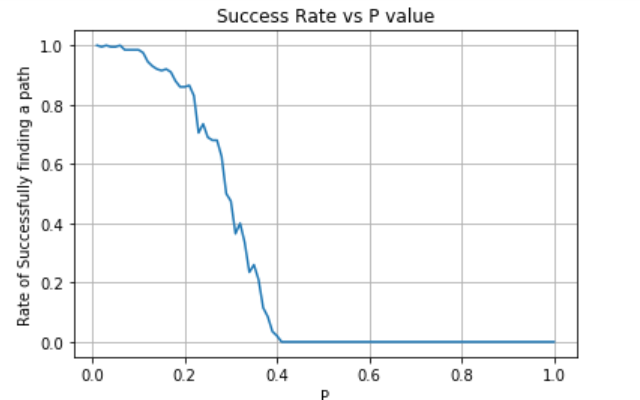
\includegraphics[width=0.3\textwidth]{../pics/question3-1.png}
\caption{\label{fig:frog}This frog was uploaded to writeLaTeX via the project menu.}
\end{figure}

\begin{thebibliography}{9}
\bibitem{nano3}
  K. Grove-Rasmussen og Jesper Nygård,
  \emph{Kvantefænomener i Nanosystemer}.
  Niels Bohr Institute \& Nano-Science Center, Københavns Universitet

\end{thebibliography}
\end{document}